\documentclass{article}

\usepackage[utf8]{inputenc}
\usepackage{graphicx}
\usepackage{caption}
\usepackage{listings}
\usepackage{lastpage}

%\usepackage[dvipsnames]{xcolor} % kolorowy tekst

\usepackage[export]{adjustbox} %center

% pakiety do języka polskiego
\usepackage[T1]{fontenc}
\usepackage[polish]{babel}
\usepackage[utf8]{inputenc}

\usepackage{indentfirst} % wcięcia

\captionsetup[figure]{name={caption}}

\title {Specyfikacja Funkcjonalna \\ Projektu ,,Game of tanks''} 
\author{Andrzej Czechowski, Bartosz Zakrzewski}
\date{Data utworzenia: 03.04.2020 \\ Data ostatniej modyfikacji: 14.04.2020}
%Termin oddania: 15.04.2020 23:59 (Środa)

% Nagłówki na każdej stronie:
\usepackage{fancyhdr}
\pagestyle{fancy}
\fancyhf{}
\rhead{Andrzej Czechowski, Bartosz Zakrzewski}
\lhead{Specyfikacja F. ,,Game of tanks''}
\rfoot{Strona \thepage \hspace{1pt} z \pageref{LastPage}}

\begin{document}
\maketitle
\thispagestyle{empty}

\clearpage

\section{Cel Projektu}
Celem projektu jest stworzenie gry zręcznościowej dla dwóch graczy, w której to zdobywa się punkty strzelając czołgiem w komórki na planszy. 

\section{Opis Teoretyczny}

\subsection{Ogólny opis gry}
\begin{enumerate}
    \item W grze rywalizuje \textbf{dwóch graczy}, którzy zdobywają punty. 
    
    \item \textbf{Plansza} składa się z pojawiających się komórek oraz dwóch czołgów umieszczonych na lewej i prawej krawędzi pola gry.
    
    \item Gracze sterują swoimi czołgami tylko wzdłuż bocznej krawędzi (do góry i do dołu). 
    
    \item Czołgi mogą strzelać pociskami poprzez obracaną \textbf{lufę}. 
    
    \item Każda pojawiająca się komórka posiada wartość od 1 do 8 (ilość żyć) oraz kolor odpowiadający maksymalnej wartości jaką komórka osiągnie w grze.
    
    \item Każde trafienie pociskiem sprawia, że komórka traci wartość (życia) o jeden.
    
    \item Gracz zyskuje punkty za uśmiercenie komórki (kiedy jego pocisk trafi w komórkę o wartości 1). Zdobywa odpowiednio tyle punktów co kolor zestrzelonej komórki.

    \item Podstawowym warunkiem wygrywania gry jest zdobycie większej ilości punktów niż drugi gracz.
        
\end{enumerate}

\subsection{Koniec gry}
Gra zakończy się gdy:
\begin{itemize}
    %\item któryś z graczy uśmierci specjalną \textbf{komórkę armagedon};
    \item jeden z graczy zdobędzie wszystkie punkty przewidziane na daną rozgrywkę (określane przy uruchamianiu gry); 
    \item upłynie określony czas (ustalany przy uruchomieniu gry). 
\end{itemize}
\par Dodatkowym warunkiem końca gry jest uśmiercenie przez gracza \textbf{komórki armagedon} i skutkuje to natychmiastową wygraną.

\subsection{Tworzenie komórek}
\begin{itemize}
    \item Przez całą grę, co \textbf{H} sekund na planszy pojawiają się \textbf{komórki} reprezentowane przez kolorowe kwadraty, w losowych miejscach. 
    
    \item Każda komórka, po stworzeniu, ma przypisaną do siebie \textbf{wartość} od \textbf{1} do \textbf{8}. 
    
    \item Komórki występują w różnych \textbf{kolorach} (i muszą być aktualizowane). Kolor jest graficzną reprezentacją największej wartości jaką miała dana komórka (jest to wskazówka dla gracza ile punktów zdobędzie).
    
    \item Dodatkowo każda komórka ma na sobie wyświetloną \textbf{aktualną wartość}, aby gracz wiedział, ile jeszcze pocisków jest potrzebne aby uśmiercić komórkę). 
    
    \item Aktualna wartość komórki, pomniejszona o jeden, określa, ile \textbf{komórek-dzieci} może się urodzić z danej komórki (np. komórka o wartości 5 może urodzić 4 komórki-dzieci). 
    
    \item Komórki-dzieci rodzą się co X sekund wokół komórki-rodzica, jeżeli jest jeszcze wolne miejsce. (,,Wokół'' oznacza kwadraty stykające się z daną komórką bokami lub wierzchołkami - każda komórka ma maksymalnie 8 sąsiadów).
    
    \item Komórki-dzieci mają przypisaną do siebie wartość \textbf{1}. 
    
    \item Przed upływem \textbf{Y} sekund wszystkie żywe komórki wzmacniają swoją siłę - ich wartość jest zwiększana o \textbf{1} (ale nie może przekroczyć \textbf{8}). 
 \end{itemize}  
    
\subsection{Zdobywanie punktów}    
\begin{itemize}

    \item Punkty za uśmiercenie komórki zdobywa ten gracz, który zada \textbf{decydujący cios} (gdy komórka ma wartość 1 i zostaje trafiona przez gracza). 
    
    \item Za uśmiercenie komórki, gracz zdobywa liczbę punktów odpowiadającą \textbf{największej wartości}, która była przypisana do tej komórki podczas gry (nie więcej niż 8) (tyle punktów ilu odpowiada kolor komórki). 
    
    \item Pod losowymi komórkami mogą pojawić się \textbf{punkty spadkowe} - bonusowe punkty.
 \end{itemize}  
    
\subsection{Punkty spadkowe}
\begin{itemize}

    \item Punkty spadkowe mogą występować w wariantach: \textbf{10}, \textbf{20}, \textbf{30}, \textbf{50}, \textbf{100}. 

    \item Punkty spadkowe występują z częstotliwością odwrotnie proporcjonalną do ich wartości, czyli punkty spadkowe \textbf{s\_10}, będą występowały częściej niż punkty spadkowe \textbf{s\_20}.

 \end{itemize}  
    
\subsection{Informacje dodatkowe}  
\begin{itemize}
    \item Komórka armagedon niczym nie wyróżnia się graficznie.
    
    \item W trakcie gry, co \textbf{Z} sekund, prędkość pocisków zwiększa się o \textbf{K} procent, a wielkość komórek ulega zmniejszeniu o \textbf{L} procent.
 \end{itemize}  
 
\subsection{Rysunki teoretyczne}

Rysunki są uproszczone i które nie przedstawiają finalnej wersji gry.
% odzwierciedlają uproszczone działanie gry. 
%Plansza nie będzie ,,szachownicą'', a kolory komórek mogą się zmienić w zależności od tego czy będą dostępne podczas implementacji.

\begin{figure} [hbt!]
    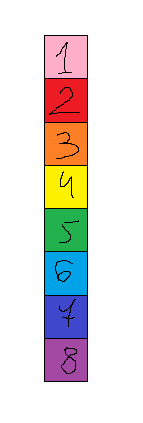
\includegraphics[width=3cm,center]{img/wartosciKomorek.png}
    \captionof{figure}{Przykładowe wartości komórek}
\end{figure}

\clearpage

\begin{figure} [hbt!]
    \includegraphics[width=12cm,center]{img/upływCzasu.png}
    \captionof{figure}{H sekund - pojawienie się komórek, X s. - rodzenie się dzieci, Y s. - wzrost wartości komórek o jeden}
\end{figure}

\clearpage

\begin{figure} [hbt!]
    \includegraphics[width=13cm,center]{img/upływCzasuK.png}
    \captionof{figure}{Rysunek gracza oraz zwiększanie się prędkości o K\% co Z sekund}
\end{figure}


\begin{figure} [hbt!]
    \includegraphics[width=8cm,center]{img/upływCzasuZ.png}
    \captionof{figure}{Zmniejszenie się rozmiaru komórek po Z sekundach o L\%}
\end{figure}

%\clearpage

\begin{figure} [hbt!]
    \includegraphics[width=10cm,center]{img/zdobywaniePunktów2.png}
    \captionof{figure}{Mechanizm zdobywania punktów}
\end{figure}

\clearpage

\section{Opis funkcjonalności}

\subsection{Możliwości programu}
    \begin{itemize}
    
    \item Grę będzie można uruchomić z wiersza poleceń.
    
    \item Gra będzie odbywać się na jednym stanowisku (komputerze) - na jednej klawiaturze będą przypisane przyciski dla poszczególnego gracza.

    \item Wszelkie stałe wartości wykorzystywane w programie będą wczytywane z \textbf{pliku konfiguracyjnego}. 
    
    \item \textbf{Końcowy stan gry} (plansza z komórkami) będzie zapisywany w formie graficznej do pliku.

    \end{itemize}

\subsection{Zmienne wczytywane z pliku wejściowego}
Domyślne wartości są przedstawione w nawiasach ().
\begin{itemize}
    \item WIDTH, HEIGTH (480, 360) - rozmiar planszy,
    \item P (10) - określa ilość pocisków jednocześnie wystrzelonych przez jeden czołg,
    \item H (5) - określa co ile sekund na planszy pojawią się nowe komórki,
    \item X (6) - określa co ile sekund wokół komórki rodzica pojawią się komórki-dzieci,
    \item Y (10) - określa co ile sekund komórki wzmacniają swoją wartość o 1,
    \item Z (20) - co tyle sekund:
        \begin{itemize}
            \item prędkość pocisków zwiększa się o K (5) procent,
            \item wielkość komórek ulega zmniejszeniu o L (10) procent,
        \end{itemize}
    \item TIME (300) - czas rozgrywki w sekundach,
    \item WIN\_SCORE (500) - punkty, które trzeba zdobyć aby wygrać rozgrywkę.
\end{itemize}
\clearpage
\subsection{Sterowanie}
Wstępne sterowanie:
\par Gracz 1: 
\begin{itemize}
    \item Ruch: W - w górę, S - w dół
    \item Strzał: SPACJA
    \item Ruch lufą: A - ruch lufy w dół, D - ruch lufy w górę
\end{itemize} 

Gracz 2: 
\begin{itemize}
    \item Ruch: STRZAŁKA W GÓRĘ - w górę, STRZAŁKA W DÓŁ - w dół
    \item Strzał: ENTER
    \item Ruch lufą:  STRZAŁKA W LEWO - ruch lufy w dół, STRZAŁKA W PRAWO - ruch lufy w górę
\end{itemize}

\subsection{Dane wejściowe}
Użytkownik musi uzupełnić plik wejściowy TXT zawierający liczby całkowite, które mają zostać wczytane. Liczby mogą być podane dowolnej kolejności, jednak przed liczbą musi być podana nazwa zmiennej, określająca do czego odnosi się ta liczba. Wartości i nazwy zmiennych muszą być oddzielone dowolnymi znakami białymi (spacją, tabulatorem, enterem lub ich kombinacją). \\

Przykładowy plik wejściowy:
\begin{lstlisting}    
WIDTH 500 
HEIGHT 500
P 10 
H 10 
X 1 
Y 6 
Z 10 
K 20 
L 5 
TIME 300 
WIN_SCORE 100
\end{lstlisting} 
\clearpage
\subsection{Dane wyjściowe}
Jedynym plikiem wyjściowym będzie plik PNG, który przedstawi stan planszy zaraz po ukończeniu gry.

\begin{figure} [hbt!]
    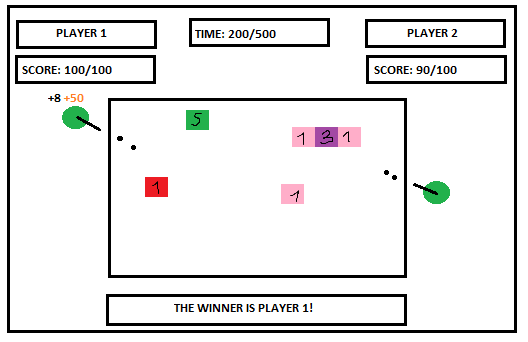
\includegraphics[width=12cm,center]{img/koncowyStanPlanszy2.png}
    \captionof{figure}{Poglądowy końcowy stan gry}
\end{figure}

\section{Scenariusz działania programu}
\begin{enumerate}

    \item Użytkownik musi pobrać kod źródłowy z repozytorium i uruchomić grę wpisując w wierszu poleceń: ,,java -jar Game\_of\_tanks.jar''. (Jeżeli zmienimy lub dodamy opcje uruchomienia poinformujemy użytkownika o tym w sprawozdaniu końcowym lub w proof of concept.)

    \item Otworzy się okienko z grą. ,,Aplikacja'' będzie miała przycisk ,,X'' po naciśnięciu którego wychodzi się z gry.

    \item Aby rozpocząć rozgrywkę należy nacisnąć przycisk Enter.
    
    \item Gra toczy się, aż któryś z warunków ukończenia gry zostanie spełniony.
    
    \item Gra oznajmia który gracz jest zwycięzcą. (Jest to warunek utworzenia pliku PNG).
    
    \item Użytkownik wyłącza grę przyciskiem ESCAPE lub zamyka otwarte okno przyciskiem X.
    
    \item Użytkownik może zobaczyć plik PNG z końcową planszą.
    
\end{enumerate}

\section{Sytuacja wyjątkowe}
\begin{itemize}
    \item Gdy użytkownik nie poda którejś ze zmiennych albo format zmiennej będzie niezgodny z ograniczeniami gry, program przepisze jej wartość domyślną.
    
    \item Gdy plik wejściowy nie będzie istniał, to wszystkie zmienne będą miały wartość domyślną.
    
    \item Gdy aplikacja wyłączy się w trakcie rozgrywki, wynik pozostanie nierozstrzygnięty - nie zapisze się plik PNG.
    
    \item Gracz nie może wyjechać swoim czołgiem za planszę - zatrzyma się w maksymalnym górnym lub dolnym położeniu planszy.
    
    \item Pocisk nie może ustrzelić kilku komórek na raz (niszczy się gdy trafi w komórkę) ani nie zada obrażeń graczowi po drugiej stronie.
    
    \item Komórki-dzieci są traktowane jak normalne komórki (tylko w trakcie pojawienia się mają wartość 1) - np. jeżeli zwiększą swoją wartość będą mogły także rodzić kolejne komórki-dzieci.
    
    
\end{itemize}

\section{Ograniczenia}

    \begin{itemize}
        \item Lufa obraca się w  zakresie $ \pm 45$ stopni od pozycji wyjściowej (w pozycji wyjściowej działo skierowane jest równolegle do \textbf{osi OX}).
        
        \item Gracz nie może mieć jednocześnie wystrzelonych więcej niż \textbf{P} pocisków.
    
        \item Komórki nie powinny nachodzić na siebie. 
    
        \item Końcowa prędkość nie może przekroczyć \textbf{300 \%} wejściowej prędkości, a komórka nie może zmaleć poniżej \textbf{50 \%} wejściowego rozmiaru. 
        
        \item Rozmiar planszy nie może być mniejszy niż (480, 360), ani większy niż (1440, 1080).
    \end{itemize}
  
\clearpage
\section{Testowanie}
Testowanie będzie odbywać się kolejno etapami podczas implementacji: 
\begin{enumerate}
    \item Tworzenie planszy i pojawianie się komórek w losowych miejscach w obszarze planszy.
    \item Właściwości komórek: rodzenie się dzieci, zwiększanie się wartości.
    \item Strzelanie, ruch pocisków.
    \item Zdobywanie punktów.
    \item Poruszanie się lufą.
    \item Poruszanie się czołgiem.
    \item Dodanie drugiego gracza.
    \item Zmniejszanie się rozmiaru komórek.
    \item Wygrywanie, komórka-armagedon, przekroczenie punktów do wygranej.
    \item Wczytywanie danych wejściowych.
    \item Tworzenie pliku PNG.
\end{enumerate}
\par Wyniki każdego z testów będą udokumentowane.

% \clearpage
\section{Źródła}

\begin{itemize}
    \item Tobiasz Siemiński - opis specyfikacji funkcjonalnej: https://sortris.blogspot.com/2010/05/jak-pisac-specyfikacje-funkcjonalna.html
     
    \item Opis teoretyczny został przedstawiony przez dr. Pawła Zawadzkiego
    
    \item Interpunkcja w wyliczeniach https://www.ekorekta24.pl/interpunkcja-w-wyliczeniach-przecinki-sredniki-a-moze-nic/
    \item Rysunki poglądowe zostały wykonane w programie Paint

    \item Ten dokument został utworzony w LaTeX'ie za pomocą strony https://www.overleaf.com
    
    \item Jest to pierwszy z kolei dokument dotyczący projektu ,,Game\_of\_tanks''
\end{itemize}

\end{document}
